\documentclass[12pt,letterpaper]{article}

\usepackage[utf8]{inputenc}
\usepackage[T1]{fontenc}
\usepackage{amsmath}
\usepackage{amsfonts}
\usepackage{amssymb}
\usepackage{amsthm}
\usepackage[left=2cm,right=2cm,top=2cm,bottom=2cm,headheight=22pt]{geometry}
\usepackage{fancyhdr}
\usepackage{setspace}
\usepackage{lastpage}
\usepackage{graphicx}
\usepackage{caption}
\usepackage{subcaption}


\theoremstyle{definition}
\newtheorem{question}{Question}
\newtheorem{example}{Example}
\newtheorem{exercise}[question]{Exercise}
\newtheorem*{challenge}{Challenge}

\begin{document}

%Paramètres de mise en forme des paragraphes selon les normes françaises
\setlength{\parskip}{1ex plus 0.5ex minus 0.2ex}
\setlength{\parindent}{0pt}

%Paramètres relatifs aux en-têtes et pieds de page.
\pagestyle{fancy}
\lhead{Theron J Hitchman}
\chead{\Large Images for Meeting 02}
\rhead{Spring 2015}
\lfoot{\emph{Math and Decision Making}}
\cfoot{}
\rfoot{\emph{\thepage\ of \pageref{LastPage}}}


\section*{Pictures for Questions 1 and 2}

\begin{figure}[h!]
    \begin{subfigure}[b]{0.4\textwidth}
        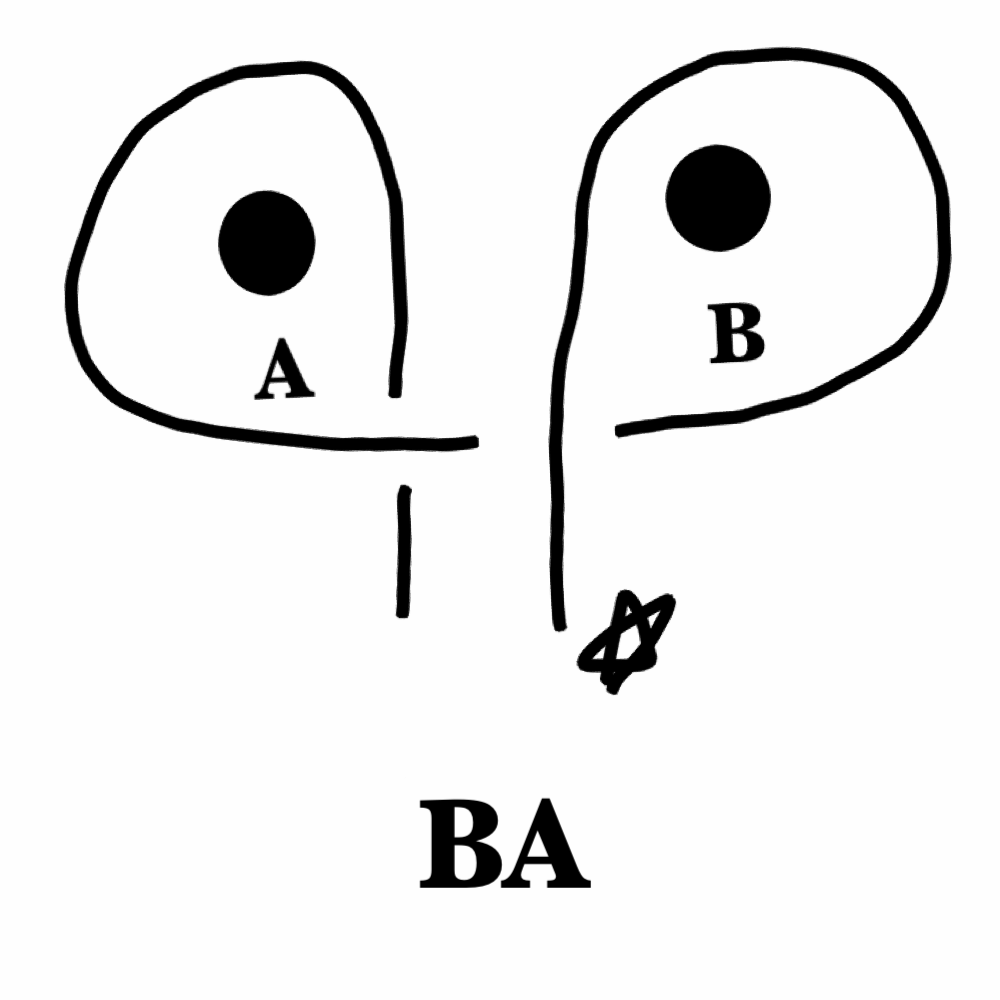
\includegraphics[width=\textwidth]{phppics/BA-label.png}
    \end{subfigure}
    \qquad
    \begin{subfigure}[b]{0.4\textwidth}
        
\includegraphics[width=\textwidth]{phppics/AsBsABs-label.png}
    \end{subfigure}
\end{figure}

\begin{figure}[h]
    
\includegraphics[height=2.5in]{phppics/AABs-badlabel.png}
\end{figure}

\clearpage


\section*{Pictures for Questions 3 and 4}

\begin{figure}[h]
    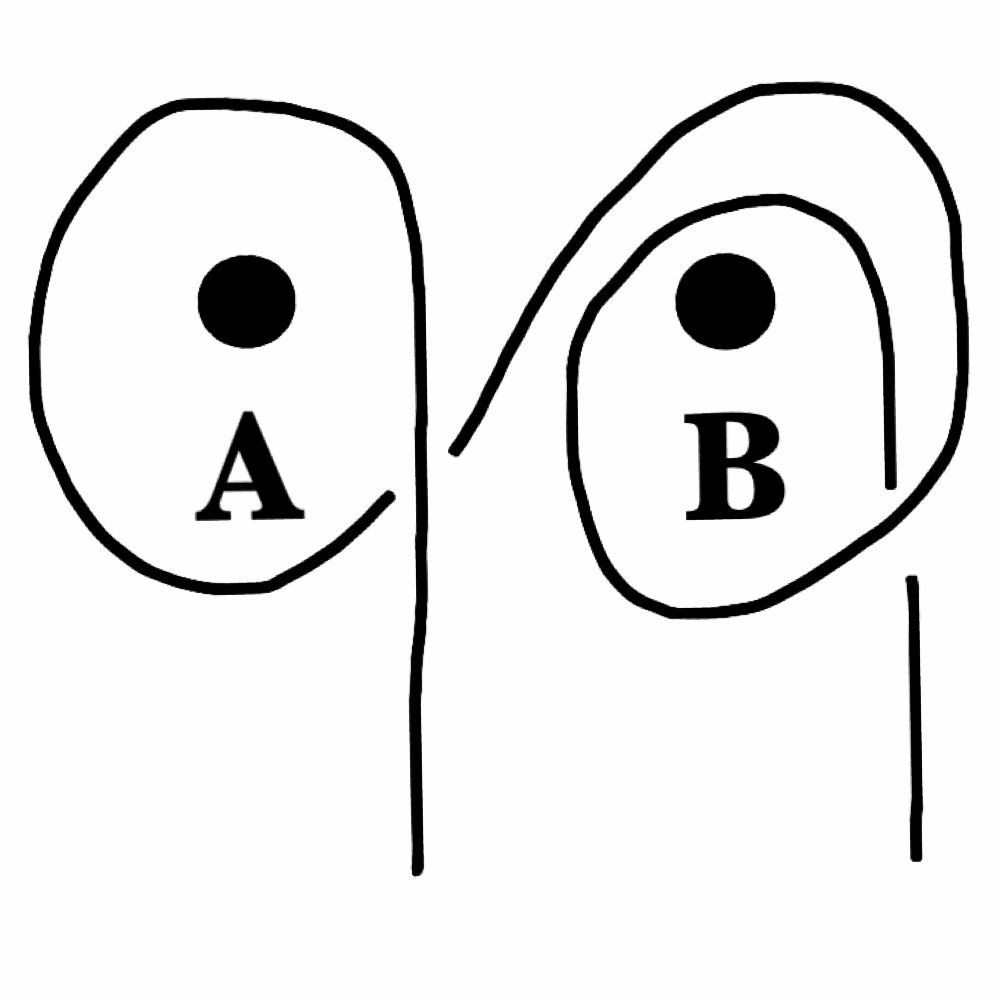
\includegraphics[height=3in]{phppics/AsBB.png}
\end{figure}

\begin{figure}[h]
    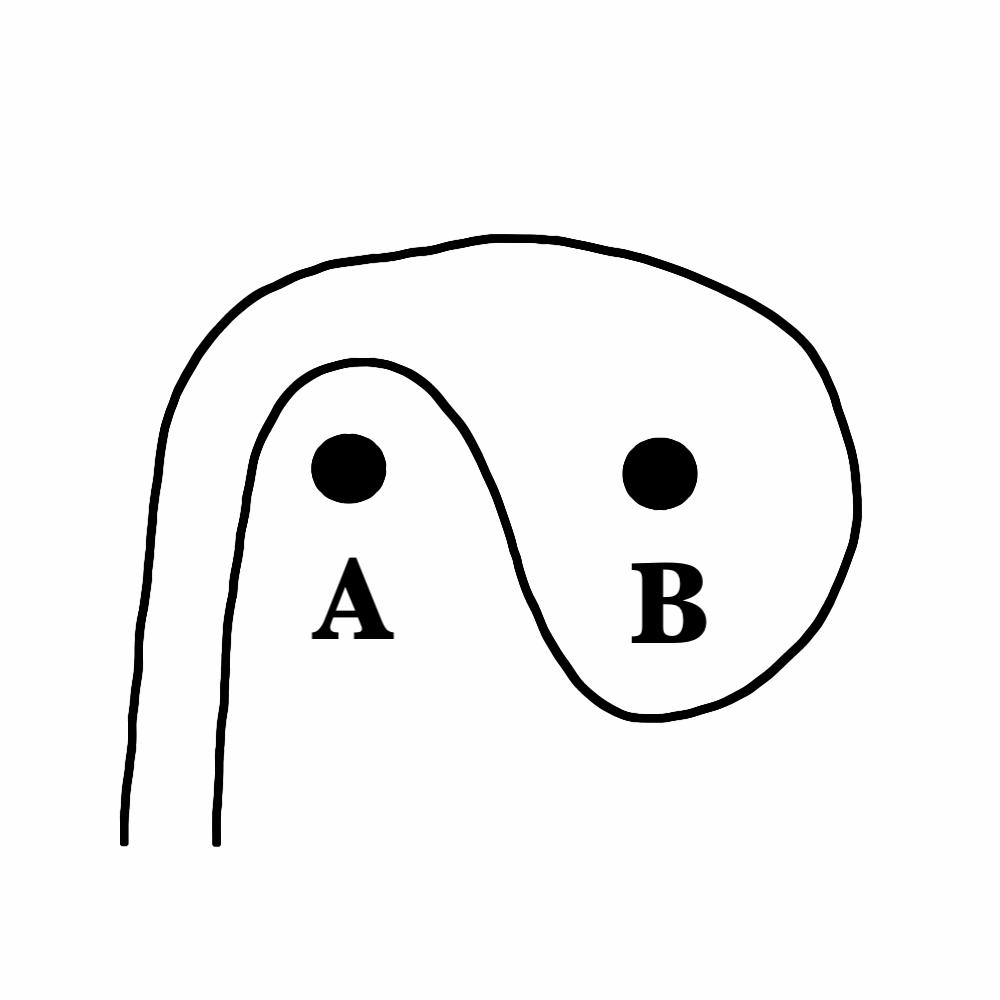
\includegraphics[height=3in]{phppics/ABAs.png}
\end{figure}


\end{document}